\documentclass{article}

\usepackage[a4paper]{geometry}
\usepackage{graphicx}
\usepackage{wrapfig}
\usepackage[utf8]{inputenc}
\usepackage[english]{babel}
\usepackage{amsmath}
\usepackage{listings}
\usepackage{amssymb}
\usepackage{amsthm}
\usepackage{bm}
\usepackage{hyperref}
\usepackage{bbm}
\usepackage{mathtools}
\usepackage{microtype}
\usepackage{enumerate}
\usepackage{upgreek}
\usepackage{float}
\usepackage{booktabs}
\usepackage{tabularx}
\usepackage{svg}
\usepackage[]{xcolor}
\usepackage{setspace}
\usepackage{pdfpages}
%\usepackage{fullpage}
\usepackage[justification=centering]{caption}
\usepackage{natbib}
\bibliographystyle{apalike}
\usepackage{titlesec}
\usepackage{import}

\newcommand{\incfig}[2][1]{%
\fontsize{15pt}{16pt}\selectfont 
    \def\svgwidth{#1\columnwidth}
    \import{./figures/}{#2.pdf_tex}
}
% \pdfsuppresswarningpagegroup=1

\newtheorem{lemma}{Lemma}[section]
\newtheorem{theorem}{Theorem}[section]
\theoremstyle{definition}
\newtheorem{definition}{Definition}[section]
\newtheorem*{definition*}{Definition}
\theoremstyle{exercise}
\newtheorem{exercise}{Exercise}[section]
\theoremstyle{remark}
\newtheorem*{remark}{Remark}

% Font
% \usepackage[T1]{fontenc}
% \usepackage[utf8]{inputenc}
% \usepackage[urw-garamond]{mathdesign}

\newcommand{\eq}{&=}
\newcommand\nt{\addtocounter{equation}{1}\tag{\theequation}}



\title{Bayesian Unit Root Testing: A Short Simulation Study}
\author{Antoine Carnec}
\date{}

\begin{document}
\maketitle
\noindent


\section*{Introduction}

Assessing whether a stochastic process is stationary is a critical part of any time series analysis, since we usually rely on theoretical guarantees that our estimators and inferences are well behaved under the assumption of stationarity.
The classical test for this is the \emph{Unit Root Test} or Dickey Fuller test, which amounts to testing the null $H_0: \varphi = 1$ against the alternative $H_1: \varphi < 1$ in the equation
\begin{align*}
y_t = \varphi y_{t-1} + \varepsilon_{t}. \nt \label{eq:DF}
\end{align*}
(We assume that $\varphi \geq 0$ for simplicity, and that the variance of $\varepsilon_{t}$ is known).


The test proceeds by estimating the OLS estimator of the coefficient $\hat{\varphi}$, from whence one can derive that
\(
    \hat{\varphi} - 1
\)
has the \emph{Dickey Fuller} distribution, whose quantiles can be readily tabulated \citep{tsay2005analysis}. Therefore a rejection region can be defined and the test is defined.

In this paper I want to investigate empirically whether there could be a Bayesian alternative to this test.
I want to investigate whether the very simple strategy of calculating the alternative hypothesis posterior $p(\varphi < 1 \;|\; \mathbf{y})$ by a sampling strategy can compete with the DF---a classic hypothesis testing approach.
I will do this simply by simulating many time series of size $T$ following an AR(1) process with coefficient $\varphi$ and $\varepsilon_{t} = \mathcal{N}(0, 1)$.
I will see if the Bayesian approach can be competitive with the Frequentist approach in this simple setting.
\cite{so1999bayesian} carry out the same strategy and find that their method performs about as well as the ADF test at moderate sample sizes. They use a Gibbs Sampler as their inference algorithm, therefore their approach is less general than the one presented here we will let Stan take care of inference for us.


\subsection*{Why be Bayesian?}
Why be Bayesian in this context?
The Bayesian approach is perfectly general from a modelling perspective. For example, if one wanted to design a Dickey-Fuller-type test for the model
\begin{align*}
    y_{t} = f(t) + \varphi y_{t-1} + \varepsilon_{t}
\end{align*}
where $f : \mathbb{R} \to \mathbb{R}$ is some arbitrary function, the practicioner must find a test statistics for every $f$ proposed.
The Bayesian however can easily incorporate this into their model simply by changing their likelihood function 
(I discuss some possible modelling extensions in the conclusion).
The tradeoff is of course that Bayesian computation is difficult, and sampling strategies are only approximate methods. I don't think this is such a big problem, as the DF test also relies on an approximation---insofar as the test statistic is asymptotically DF-distributed. The Bayesian approach has no problem with low $T$, and the accuracy of the Monte Carlo estimator can be increased by increasing $N$ (equivalently running the inference algorithm for longer).

\subsection*{What's wrong with the unit root test?}%

A very small $p$-value only tells the statistician that there is some level of surprise.
It certainly is not true that small $p$ value in the DF test implies the rejection of the \emph{scientific hypothesis} that $\varphi=1$.
Perhaps there is a small $p$ value because the DF equation \cite{eq:DF} is misspecified.
If we do suspect a misspecification in the model, it is not so easy to change the model that much, since the ADF test is derived for 
specific functional forms of \cite{eq:DF}.

\section*{A Bayesian Approach}%

Bayesian Statistics uses characterizes a model with \emph{prior} probability distributions on the model parameters $\bm{\theta}$ and a specifies a \emph{likelihood} $p(\mathbf{y} \;|\; \bm{\theta})$, which captures how likely the data $\mathbf{\bm{y}}$ is given a certain configurations of the parameters. Having specified these, we can recover the conditional distribution of the parameters given the data we have using Bayes Theorem
\begin{align*}
    p(\bm{\theta} \;|\; \mathbf{y}) = \frac{p(\mathbf{y} \;|\; \bm{\theta})  p(\bm{\theta})}{\int_{}^{}  p(\mathbf{y} \;|\; \bm{\theta})  p(\bm{\theta}) d\bm{\theta}} \propto p(\mathbf{y} \;|\; \bm{\theta})  p(\bm{\theta}).
\end{align*}
Given that the likelihood correctly specifies the data generating distribution and that the prior accurately represents the statisticians prior beliefs, $p(\bm{\theta} \;|\; \mathbf{y})$ captures the beliefs that the statistician should have about the parameter.

In the case of our AR(1) model, let $\bm{\theta} = \varphi$. The model we use is
\begin{align*}
    p(\varphi \;|\; \mathbf{y}) \propto \prod_{t=2}^{T} \mathcal{N}(\varphi y_{t-1}, \sigma^2_{\varepsilon}) \cdot p(\varphi) \nt \label{eq:bm}
\end{align*}
where we take $\sigma^2_{\varepsilon}$ as observed for simplicity, $p(\varphi)$ is the prior distribution we set on $\bm{\varphi}$.

Now \autoref{eq:bm} gives us the posterior up to a normalising constant. In general it is very hard to calculate this normalising constant, and therefore we choose to sample from this distribution. This can easily be done with the Stan probabilistic programming language \citep{bleepbleep}. Given a generative model such as (\ref{eq:bm}), Stan allows the user to sample from the posterior using Hamiltonian Monte Carlo, % (TODO citations
which is a state of the art MCMC technique which tends to scale well with dimension\footnote{many caveats could be made here, I refer the reader to \cite{betancourt2017conceptual} for a discussion}.
We include the Stan code to implement (\ref{eq:bm}) in the appendix. I also set the number of samples to $N=5000$ and use the NUTS HMC sampler.

Given a sample $\{x_n\}_{n=1}^{N}$ of $p(\varphi \;|\; \mathbf{y})$, we can estimate
\(
    \mathbb{E}_{\varphi \;|\; \mathbf{y}}\left[f\right]
    \)
for any function $f$. This estimate is consistent and unbiased.
In particular we are interested in the probability that $\varphi < 1$, which we can recover by
\begin{align*}
    \frac{1}{N}\sum_{n=1}^{N} \mathbbm{1}(x_n < 1)  \to P(\varphi < 1 \;|\; \mathbf{y}), \text{ as } N \to \infty
\end{align*}

Our Bayesian Hypotheses will be 
\begin{align*}
    H_0: \varphi < 1 \quad H_1: \varphi \geq 1.
\end{align*}


We still have not yet show how know $p(H_1 \;|\; \mathbf{y}) := p(\varphi < 1 \;|\; \mathbf{y})$ leads to a decision---that is, do we reject the null?
Here we reject the null if $p(H_1 \;|\; \mathbf{y}) > p(H_0 \;|\; \mathbf{y})$, this is the same decision rule used in \citep{so1999bayesian}.

\section*{Prior for $\varphi$}%
An important question is which prior to set for $\varphi$.
Generally, there are four approaches to choosing this prior. A convenient choice of prior (one which leads to closed form expressions for the posterior), a non-informative or weakly-informative prior (priors which don't enforce little to no regularization), objective priors (priors which can be deduced from theoretical arguments) and subjective priors (priors which encode the statisticians prior beliefs). % TODO CITE BA 

In this paper we consider two simple priors.
A weakly informative prior, more specifically $\varphi \sim \mathcal{N}(\frac{1}{2}, 1)$. This prior ensures that $\varphi$ has density over the space where we believe it will be between---that is between $0$ and some number greater than $1$---but that it does not have much mass at $\varphi = 5$ for example\footnote{If $\varphi = 5$, then simply looking at the time series would tell you that it's not stationary}.

We consider a prior that is relatively strongly concentrated around $1$. This reflects the fact that researchers may have a strong consensus prior belief that the time series is a random walk (using arguments such as the Efficient Market Hypothesis for example).
To encode this, we set the prior to a $\text{Laplace}(1,0.1)$ distribution.

The priors are plotted in \autoref{eq:priors}.

\section*{Simulations}%

How should we compare the two procedures?
%
Well, it is described in \cite{benjamin2019three} that a given a $p$-value, we can calculate a tight upper bound on the posterior probability of the null hypothesis simply with
\begin{align*}
    p^U(H_1 \;|\; \mathbf{y}, p) = \frac{BFU}{1 + BFU}, \quad BFU = \frac{1}{-ep\log (p)}
\end{align*}
Hence we perform a direct comparison between posterior probabilities for the two priors with the posterior probability upper bound for $T \in \{ 50, 500\}$.
Note that we 

We plot the results in \autoref{fig:posterior_probs} and \ref{fig:pp2}.

\begin{figure}[H]
\centering
    \begin{minipage}{.5\textwidth}
        \centering
        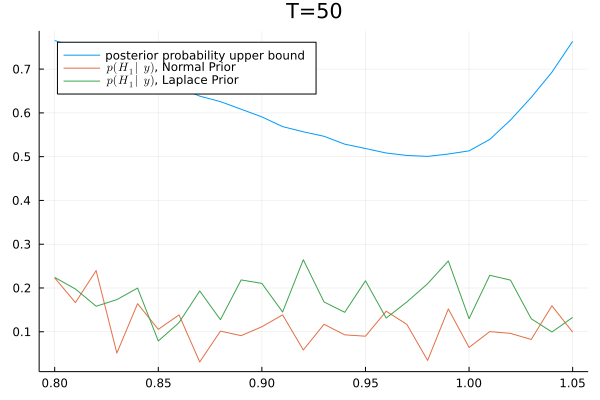
\includegraphics[width=.95\linewidth]{./plots/posterior_probs_50.png}
    \end{minipage}%
    \begin{minipage}{.5\textwidth}
        \centering
        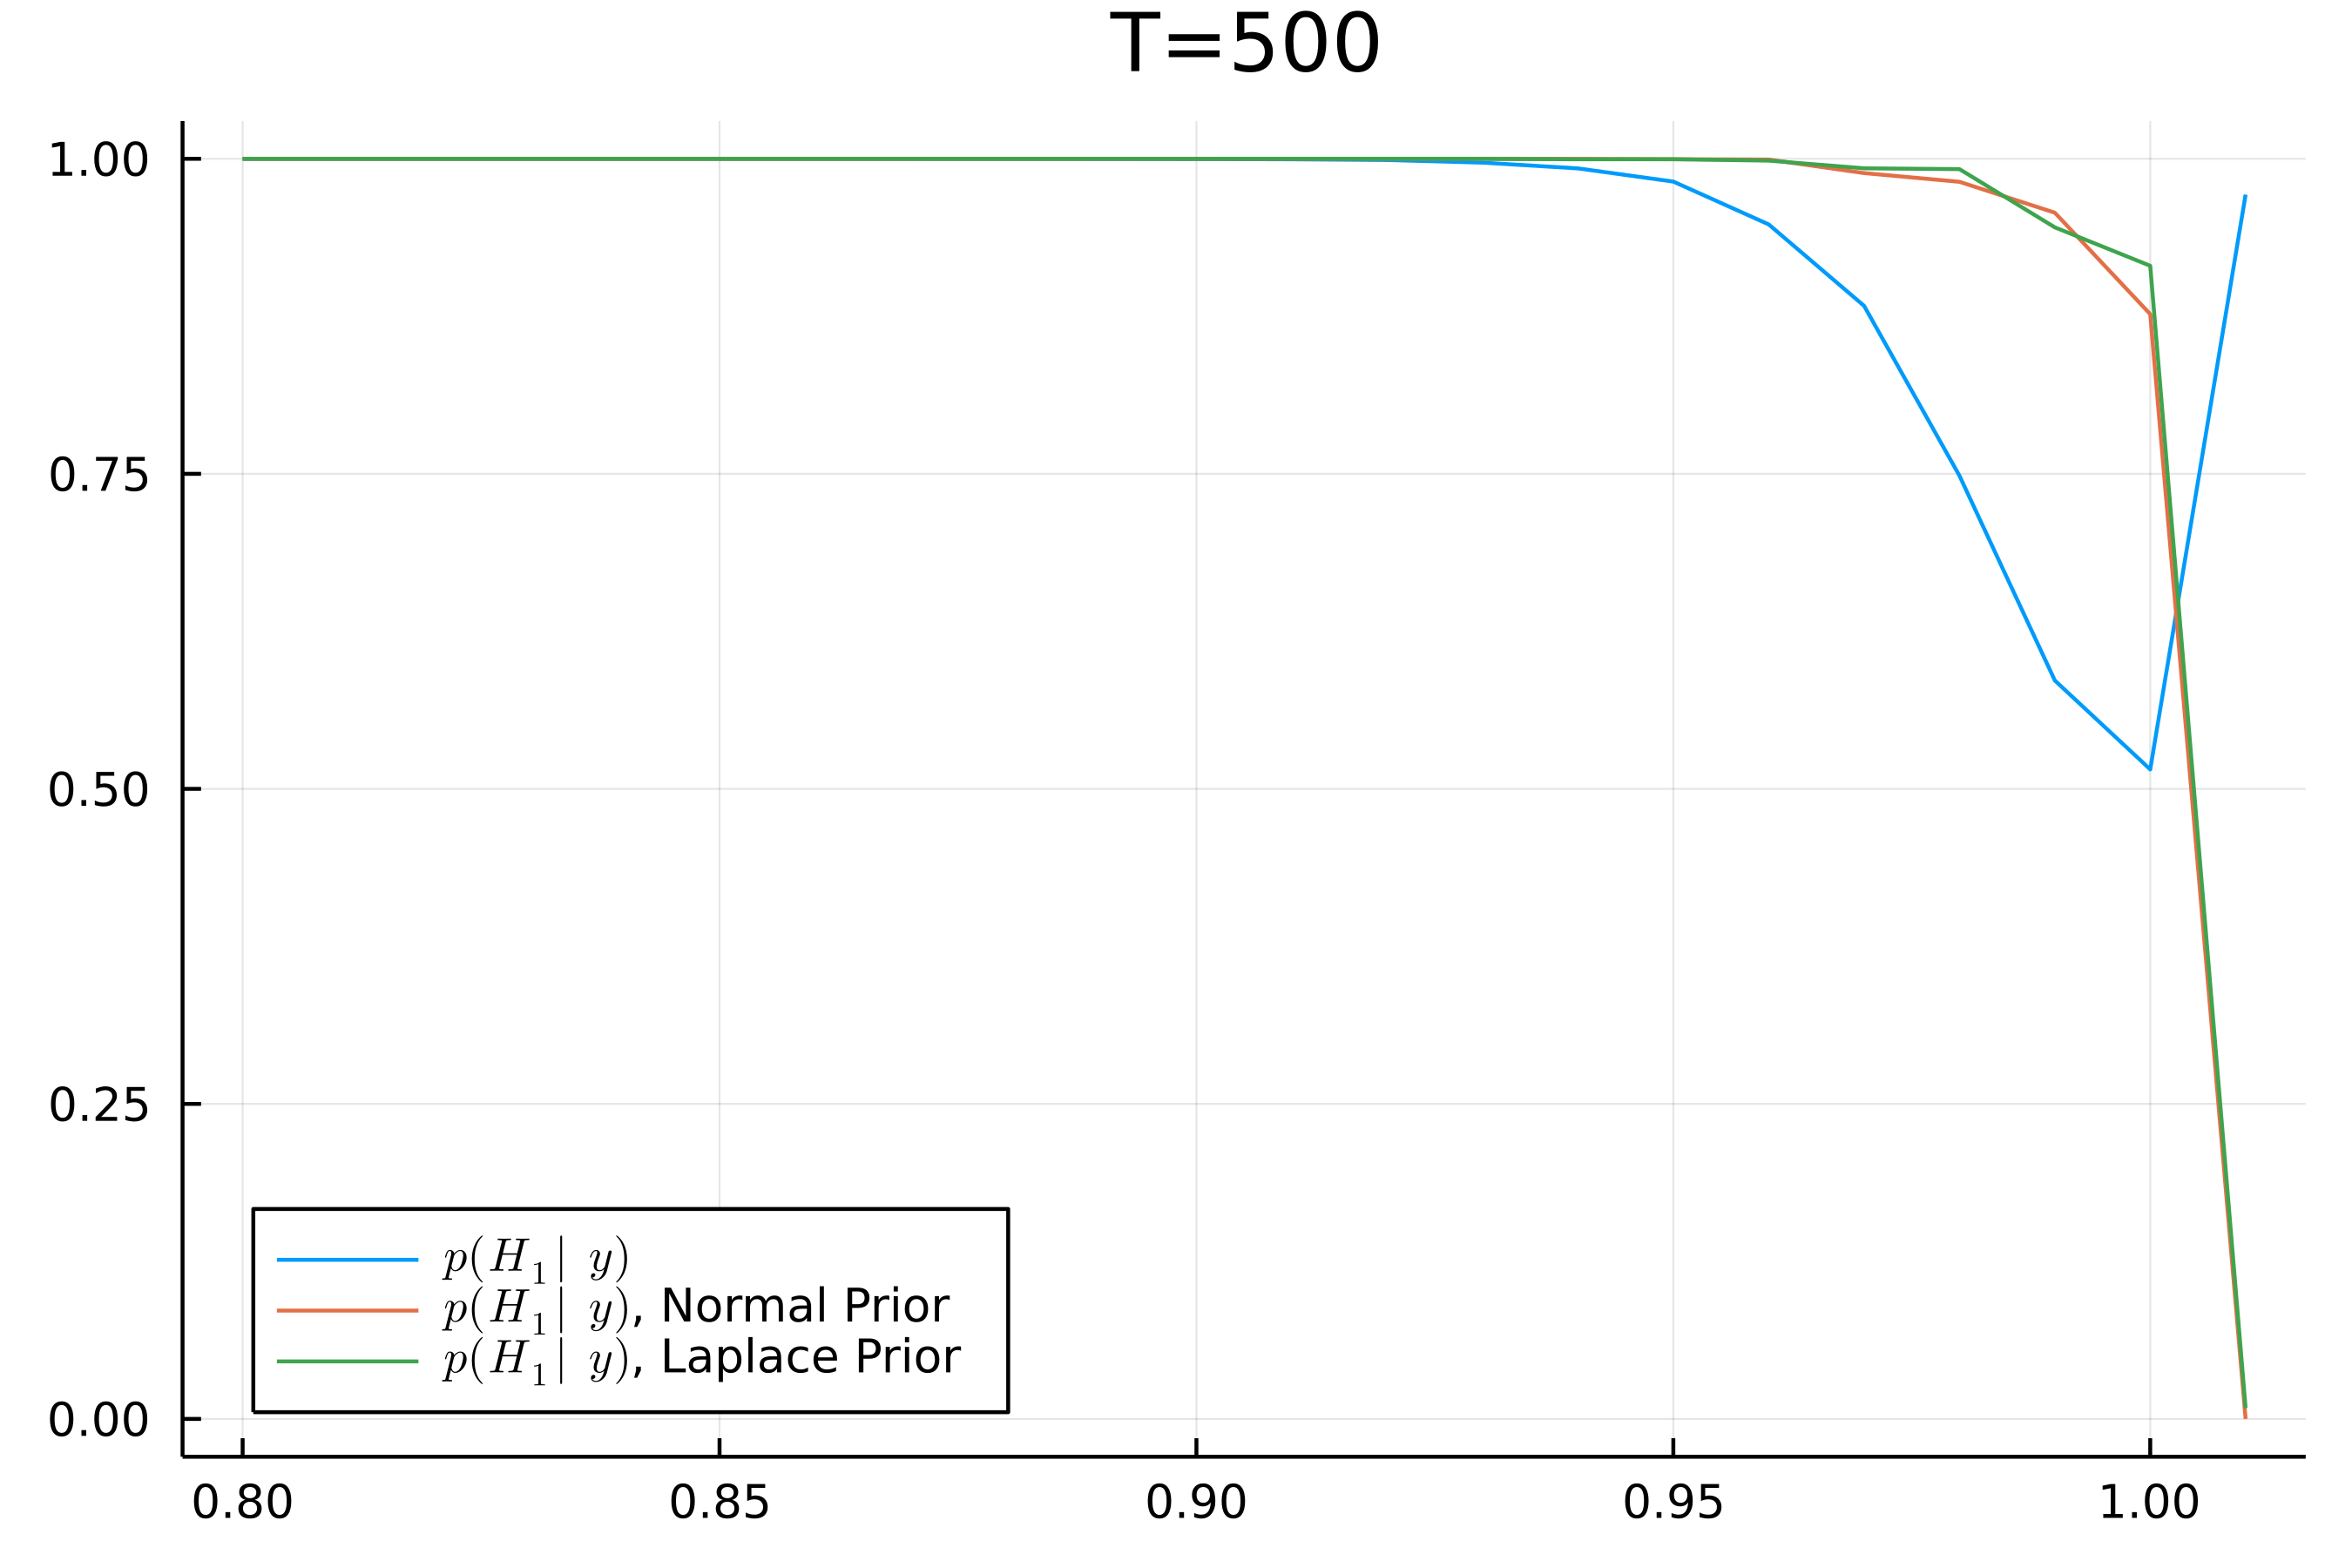
\includegraphics[width=.95\linewidth]{./plots/posterior_probs_500.png}
    \end{minipage}
        \captionof{figure}{$\varphi$ on the $x$ axis, plotted from $0$ to $1.01$}
        \label{fig:posterior_probs}
\end{figure}
\begin{figure}[htpb]
    \centering
    {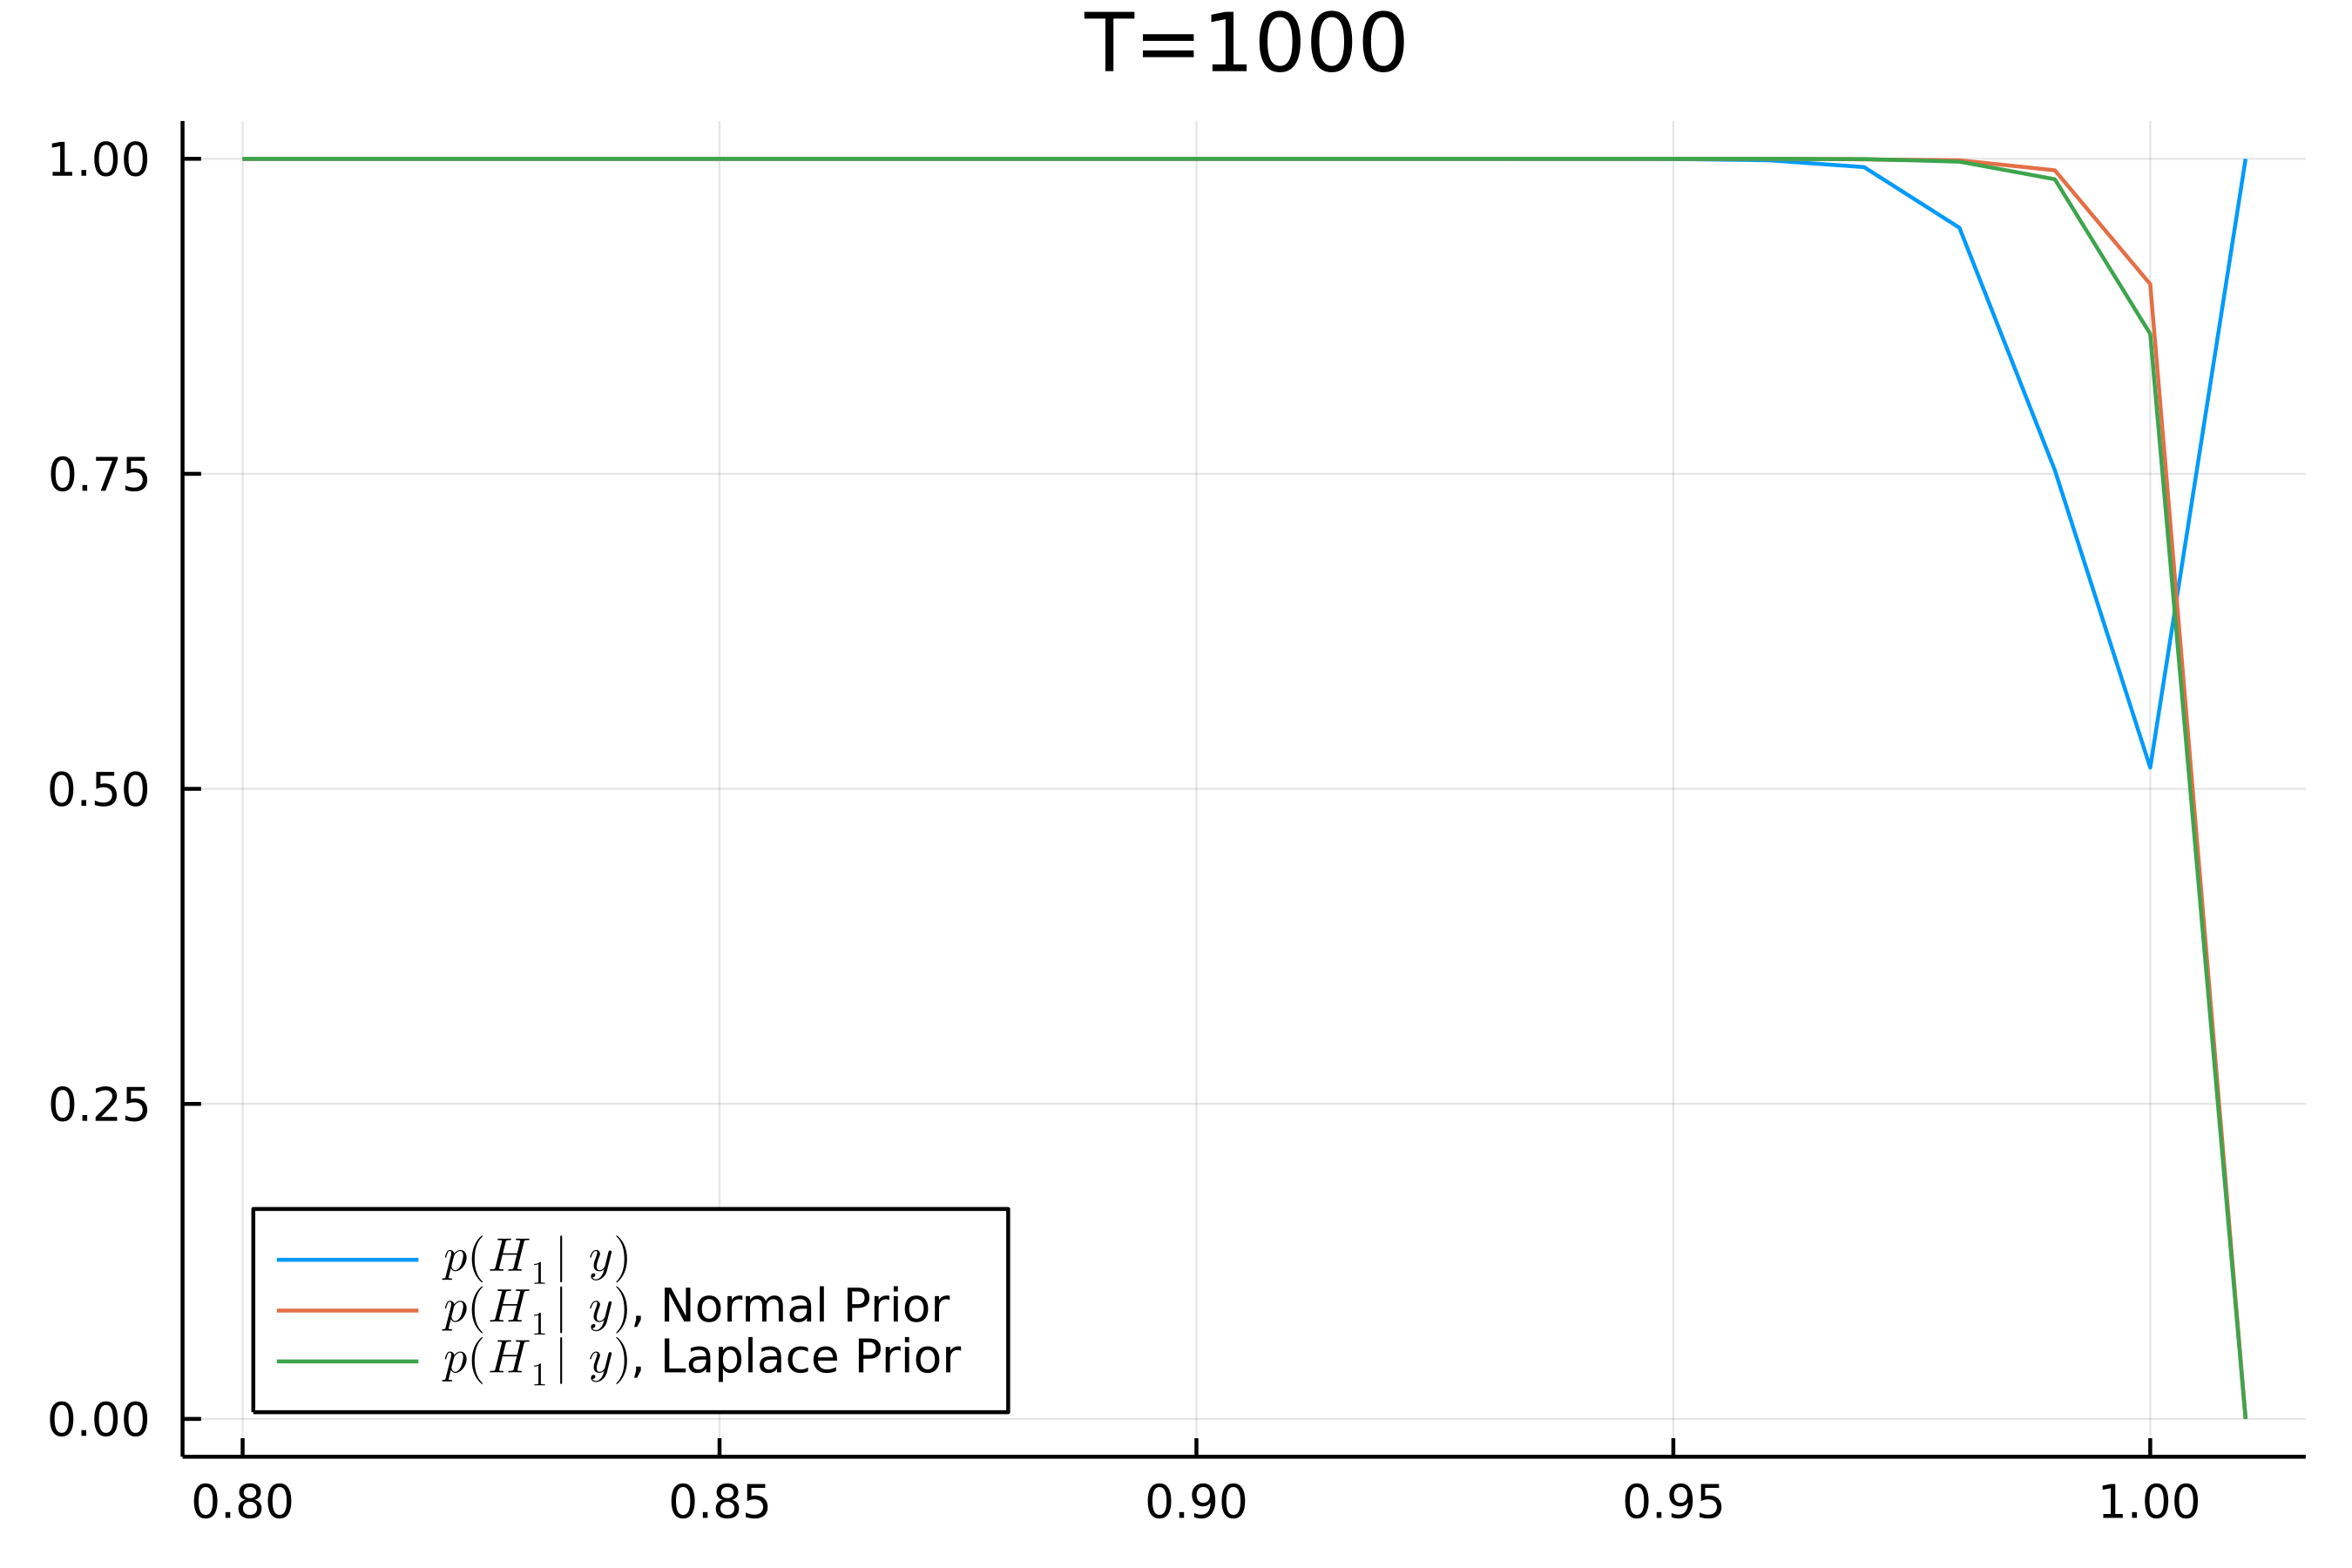
\includegraphics[width=0.8\textwidth]{./plots/posterior_probs_1000.png}}
    \caption{$\varphi$ on the $x$ axis, plotted from $0$ to $1.01$}
    \label{fig:pp2}
\end{figure}

Looking at $T=50$, we can see that there are not enough data points to really bring down the posterior probability at $\varphi = 1$. This is supported by what we see when $T=500$ which does a better job.
We can see that even the upper pound of the $DF$ test does not give the same confidence when $\varphi < 1$. However, there is obviously overconfidence here, since at $\varphi = 1$ the posterior distributions do not fall sufficiently fast enough---even for $T=1000$. From these figures above we definitely cannot endorse the Bayesian approach.
On the other hand, we can notice that the Bayesian methods still "get it right" at $\varphi = 0.99$ for example, improving upon the loss of power near $1$ that the DF test suffers from.
However, when $\varphi = 1$ the proposed method does not identify the process as stationary.


Let's verify that last claim. Let $T = 5000$.
We will simulate $50$ AR(1) process with some $\varphi$ and run all of the hypothesis decision rules, with an $\alpha = 0.05$. Recall that for the Bayesian methods we reject the null if $p(H_1 \;|\; \mathbf{y}) > 0.5)$.
We show the proportion of times the procedures made the correct choice.

\begin{table}[H]
\centering
\begin{tabular}{lllll}
    \toprule
 & $\varphi=0.95$ & $\varphi=0.99$ & $\varphi=1$ &  \\ \midrule
$DF$ test      & 1 & 1 &  1 &  \\
 Normal Prior  & 1 & 1 &  0.04 &  \\
Laplace Prior  & 1 & 1 &  0.02 & 
\end{tabular}
    \caption{$T$ = $5000$, $50$ AR1 processes run, $\alpha$ = $0.05$}
    \label{tab}
\end{table}

As \autoref{tab} shows, the Bayesian unit tests failed pretty miserably, while the DF test got everything right.


\section*{How could this analysis be extended?}%

We saw in the results that the Bayesian Hypothesis test didn't perform very well at all. Perhaps we could employ better priors on our Hypotheses. An interesting approach might be to implement \cite{johnson2010use} Non Local Prior approach to Bayesian hypothesis testing.
For these special priors, the authors prove that the Bayes Factors converge at a very fast rate, even exponential under some conditions.

Another interesting idea is the following. From a decision making standpoint, we are primarily interested in $p(\varphi_{1} = 1)$. However, it's difficult to estimate using simulations since we will never sample $1$ exactly.
A Sequential Monte Carlo sampler \citep{del2006sequential} could be designed, inspired by the rare event SMC techniques existing in the literature. The idea is to sample from a sequence of distributions such that the support of these distributions closes in on a small interval around $1$.


% Well, we know that the augmented Dickey-Fuller test allows for more non-linear dependence relations.
% Current frequentist approaches are rule-of-thumbs, which may work in practice but have little theoretical backing.

% The Bayesian approach is quite general. 
% We could perform model selection on the dependence structure of the model, using Bayesian Variable Selection.
% \begin{align*}
%     y_{t} = \varphi_1 y_{t-1} + \sum_{k=2}^{p} \varphi_{k} y_{t-k} + \varepsilon_{t}
% \end{align*}


% Another extensions, non-local priors. Very good frequentist properties.

\newpage
\section*{Stan Code}
Note, we employ a common technique when using HMC by standardizing $y$ as a preprocessing step.
This is know to (sometimes) make inference work better \citep{gelman1995bayesian}.
\subsubsection*{Weakly Informative Prior}
\begin{verbatim}
    data {
      int<lower=0> T;
      real<lower=0> sigma;
      vector[T] y;
    }
    transformed data {
      real<lower=0> sigma_std;
      vector[T] y_std;
      y_std = (y - mean(y)) / sd(y);
      sigma_std = sigma / sd(y) ;
    }
    parameters {
      real phi;
    }
    model {
      phi ~ normal(1/2, 1) ;
      y_std[2:T] ~ normal(phi * y_std[1:(T - 1)], sigma_std);
    }
\end{verbatim}
\subsubsection*{Laplace Prior}
\begin{verbatim}
    data {
      int<lower=0> T;
      real<lower=0> sigma;
      vector[T] y;
    }
    transformed data {
      real<lower=0> sigma_std;
      vector[T] y_std;
      y_std = (y - mean(y)) / sd(y);
      sigma_std = sigma / sd(y) ;
    }
    parameters {
      real phi;
    }
    model {
      phi ~ double_exponential(1, 0.1);
      y_std[2:T] ~ normal(phi * y_std[1:(T - 1)], sigma_std);
    }
\end{verbatim}
\section{Extra Figures}%
\begin{figure}[H]
    \centering
    {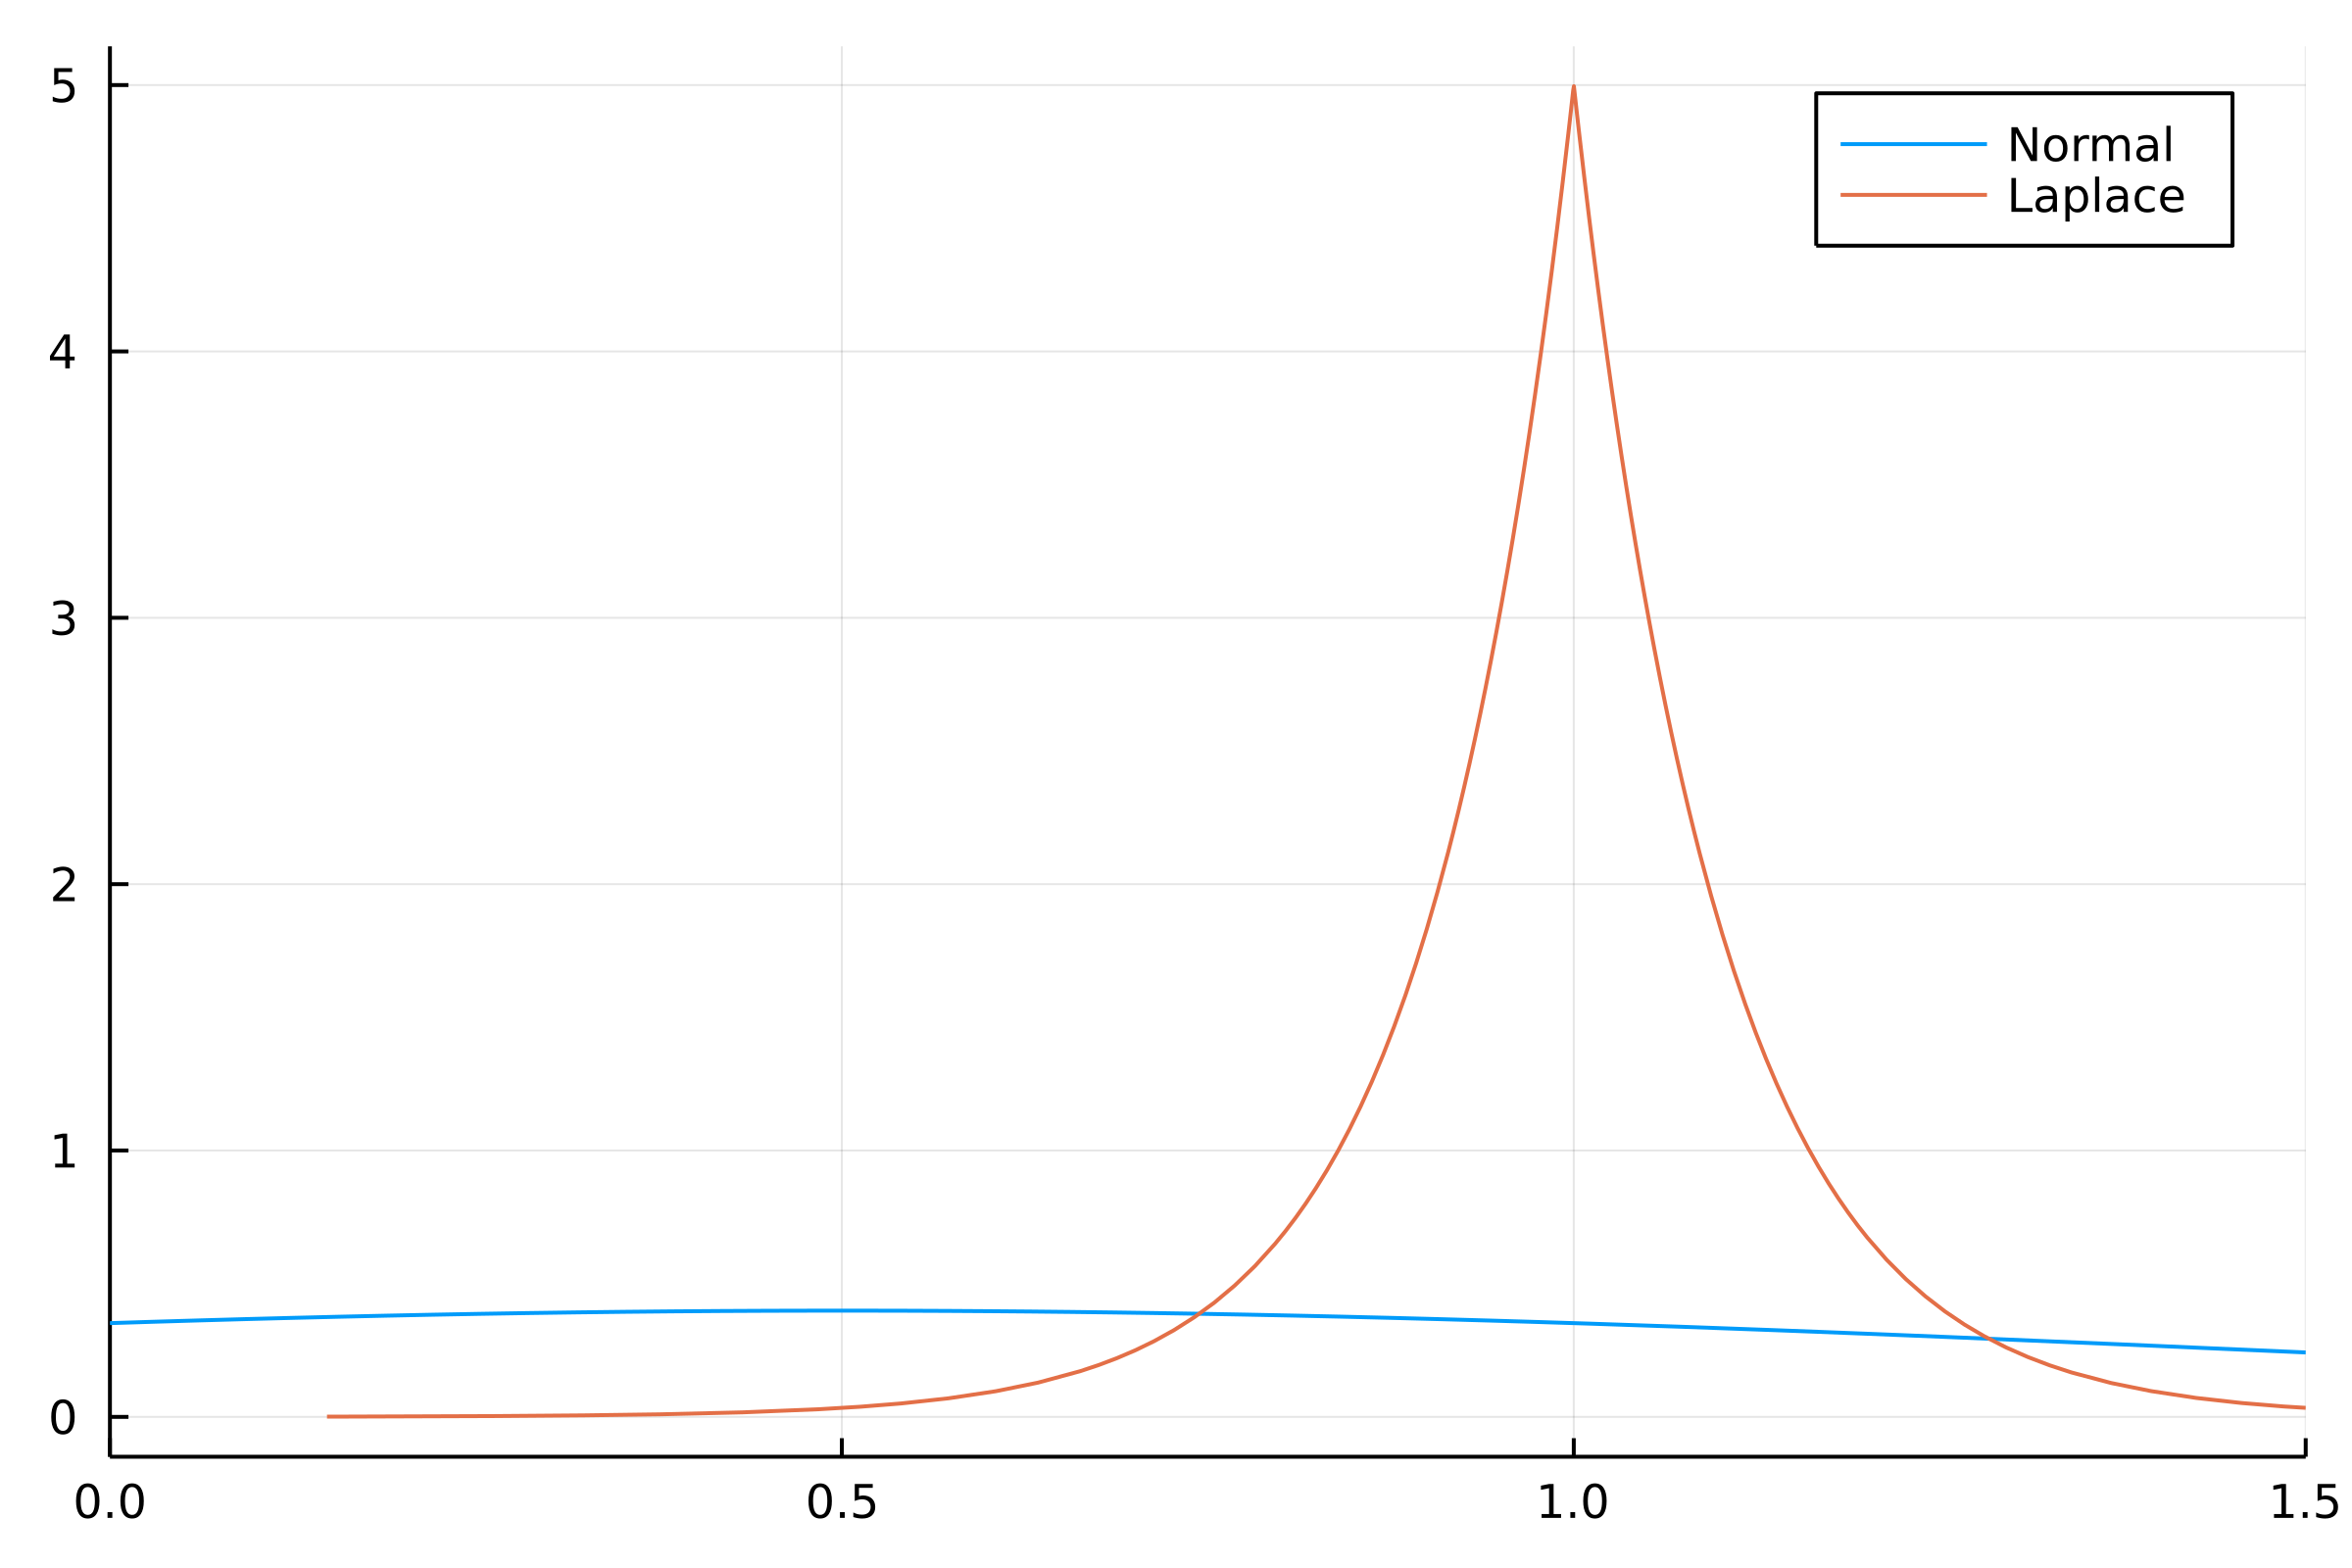
\includegraphics[width=0.8\textwidth]{./plots/priors.png}}
    \caption{The two priors used}
    \label{eq:priors}
\end{figure}


%\newpage
\bibliography{./refs.bib}
\end{document}
